\documentclass{llncs}

\usepackage{hyperref}
\usepackage{graphicx}
\usepackage{listings}

\begin{document}

\title{A linked open data architecture for contemporary historical archives}  
\author{Alexandre Rademaker\inst{1} 
  \and Suemi Higuchi\inst{2}
  \and D\'ario Augusto Borges Oliveira\inst{2}}
\institute{IBM Research and FGV/EMAp \and FGV/CPDOC}
\maketitle

\begin{abstract}
  We present a novelty architecture for historical archives maintenance
  based on Open Linked Data principles and open source distributed
  development model and tools. The presented architecture is being
  implemented as a ``proof of concept'' for the archives of the Center
  for Research and Documentation of Contemporary History of Brazil
  (CPDOC) from Getulio Vargas Foundation (FGV).
\end{abstract}

\section{Introduction}

% 1. the use of open/linked data vs. relational data
% 2. embracing the open source development model for data maintainnability
% 3. CPDOC ownership versus curatorship of the datasets

The Center for Research and Documentation of Contemporary History of
Brazil (CPDOC) of Getulio Vargas Foundation (FGV) is an institution
dedicated to the study and preservation of the Brazil recent memory,
CPDOC holds rich collections of documents organized in three major
archives. During the 70's and 80's, CPDOC team developed its own
methodology for organizing and indexing documents about contemporary
history, recognized as innovative methodology by leading educational
and research institutions. However, new technologies and trends for
data sharing and interoperability of collections suggest that a review
is needed in CPDOC processes. It is time to adjust CPDOC methodology 
to new paradigms.

CPDOC is aware of that the process of digitalization and globalization
of our society requires new methods of learning, teaching, acquiring,
storing and using informations as so to transform it into
actionable knowledge. In this scenario, FGV is uniquely positioned to
lead in this new reality, being a youthful and nimble knowledge-based
institution.

% Even though it is about the same universe of discourse -- the
% contemporary history of Brazil -- three different information systems
% were built to store the different types of documents.

In the current state, CPDOC main concern is that its archives are not
following any standard open data model. This scenario does not help to
make the CPDOC's archives widely visible online and interoperable with
other digital archives. Thus, queries to CPDOC's collections are
limited to what CPDOC systems can offer and service providers could
not use CPDOC collections in their services that could potentially
reach a wide audience.

The CPDOC's archives are maintained in three different information
systems based on traditional relational data models. The current CPDOC
infrastructure are difficult to maintain, improve and refine. The
information systems do not provide an intuitive and effective
interfaces to their users, making the access to information difficult
and limited.

% There is much talk in Brazilian leading intellectual circles of
% connecting and relating to external centers of excellence, but if
% the mechanisms of interaction are kept restricted to the old models
% (traditional professorships and visiting lectureships for a year for
% well-established professors), the interaction with the more dynamic
% sectors such as entrepreneurs and incubators of start-up companies,
% will not develop at the pace it needs to.

This article presents a research project that aims to change the
CPDOC's posture regarding its methodology and archives
maintenance. The project is an ongoing initiative to build a model of
data organization and storage that ensures easy access,
interoperability and reuse by service providers. The project proposal
is inspired by: (1) Open Data Initiative
principles~\footnote{\url{http://www.opendatainitiative.org}}; (2)
distributed open source development model and tools for easy data
management and maintenance; (3) a growing importance of data curation
concepts and practices for online digital archives management and
long-term preservation.

The project started with the objective of creating a linked open data
version of CPDOC's archives and a prototype simple and intuitive web
interface for browsing the archives. The uses of Linked Open Data
concept in line with the three laws first published by David
Eaves~\cite{3-law} and now widely accepted: (1) If it can't be
spidered or indexed, it doesn't exist; (2) If it isn't available in
open and machine readable format, it can't engage; and (3) If a legal
framework doesn't allow it to be repurposed, it doesn't empower.

We believe that CPDOC must review its methodology for digital data
maintenance, storage, preservation and access policies. If CPDOC
starts focus on the production and distribution of data and no longer
in elaborated information systems and query interfaces, CPDOC will
allow other forms of access, and therefore, new uses for these data,
regardless of CPDOC's intervention.

Our idea follows the spirit of free data preached by the Semantic Web
community in an effort to build a global network of interconnected
data. In this approach the possibility of discovering new knowledge is
unlimited and is directly consequence of the accessibility and open
standards formats adoption. Among the initiatives of this project we
emphasize the construction of a RDF~\cite{rdf-primer} data from data
originally stored in a relational database and the construction of
OWL~\cite{owl} ontologies able to make the collection of the data
source in CPDOC well defined and interoperable. The proposal is to
make the whole archive also available for download as versioned dumps
following DBPedia~\footnote{\url{http://dbpedia.org}} approach.

In the end, the project aims to stabilized CPDOC as a content
provider and curator. Thus, the goal is to develop a real effort from
a research experience making CPDOC a reference in the field of
historic preservation and documentation in Brazil.


\section{CPDOC information systems}

% CPDOC is a major center for teaching and research in the social
% sciences and contemporary history and is located in Rio de
% Janeiro. CPDOC is also a leading historical research institute in the
% country and it holds a major collection of personal archives, oral
% histories and audiovisual sources pertaining to Brazilian contemporary
% history.  CPDOC's private historical archival program hosts more than
% 1,8 million documents ranging from politics to economics, cultural
% history to social movements, and public policy to foreign
% relations. Over the years \mbox{CPDOC} has gathered a massive
% collection of oral histories. The historical archival program is
% mainly composed of three major information systems:

% \begin{itemize}
% \item Personal Archives: About 200 archival collections, comprising
%   approximately 1,8 million documents, including text, images and
%   videos.
% \item Oral History Program: A large set of testimonies (in audio and
%   video) consisting of more than 1.000 interviews, which corresponds
%   to roughly five thousand hours of recordings.
% \item Brazilian Historical Biographic Dictionary (DHBB): in the
%   current version, it consists of 7.553 entries, of which 6.584 are of
%   a biographical nature and 969 related to institutions, events and
%   concepts of interest for Brazilian history after 1930.
% \end{itemize}

% That is, the CPDOC data collection is storage in three distinct
% information systems developed originally for query and maintainance of
% three different databases. Each of these systems has independent
% management and adopts idiosyncratic criteria for the organization and
% indexing of your information. The data model vary according to the
% specific content of that they hold.

The CPDOC archives are organized in three different information
systems that share a common relational database. Each of them has an
independent management and adopts idiosyncratic criteria concerning
the organization and indexing of their information, which vary
depending on the specifications of the content they host: personal
archives, oral history interviews and the Brazilian
Historical-Biographic Dictionary. Each of them is briefly described in
the following subsections.

\subsection{Personal Archives (Acessus)}

Historical documents, in the most varied textual and audiovisual
supports, are precious sources of knowledge that help us to know
deeper our history. They can be manuscripts, diaries, letters,
photography, speeches or memos and whenever they compose personal
files of people that influenced the political and social scenario of
our country, they represent much more than private memories: they are
concrete registry of a collective memory.

Currently, more than 200 personal archives that belonged to
presidents, ministers, military personal and other important people to
the Brazilian society compose the CPDOC collections. Together, they
comprise nearly 1.8 million documents or 5.2 millions pages. From
this, nearly 700 thousands pages are digitalized and the expectance is
to digitalize the whole collection in the next years. The metadata of
the collection is stored in a system called \emph{Acessus} that allows
queries to database using some basic search interface which support
only keywords queries to a specific database fields defined in an
\emph{ad hoc} manner.

The Acessus system consist of: an intranet web interface for data
manipulation and reports generation; a set of tables in the CPDOC
shared relational database; and (3) directories in a file system where
the actual files of digitalized documents are saved.

\subsection{Oral History Interviews (PO)}

The CPDOC collection of Oral History comprises currently more than
6.000 hours of recording, corresponding to nearly 2.000
interviews. More than 90\%, video or audio, are in digital format. For
the time being, two kinds of query are available in the database:
query by subject and query by interviewed. Each interview record holds
a brief technical information and a summary with the descriptions of
the interview themes in the order they appear during the record. Only
10\% of the interviews are transcribed, but to access the audio/video
content the user is requested to come personally to CPDOC. Currently
CPDOC is analyzing better ways of making this data available online,
considering different aspects such as the best format, use policies,
access control and copyrights for each interview.

The \emph{PO} system consist of: an intranet web interface for data
manipulation and reports generation; a set of tables in the CPDOC
shared relational database; and (3) directories in a file system where
the actual files of digitalized audio and video interviews are saved.


\subsection{Brazilian Historical-Biographic Dictionary (DHBB)}

The Brazilian Historical-Biographic Dictionary (DHBB) is certainly one
of the main collections about Brazilian historical politicians and
themes after 1930. It hosts more than 7.500 entries of biographic and
thematic nature, that means, people, institutions, organizations and
events carefully selected using criteria that measure the relevance of
those to the political history for the given period. The dictionary
database stores a few metadata concerning each entry, and the query is
limited to the title or occurrence of words within the text. 

The DHBB system consist of: an intranet web interface for data
manipulation and reports generation; and a set of tables in the CPDOC
shared relational database.


\subsection{CPDOC portal and public access interface}

The three CPDOC systems share a common relational database for a
simple reason. The idea was to facilitate the construction of a single
query interface over all CPDOC archives.

In the CPDOC web portal, the user is required to log into the system
in order to access data and the use of the available GUI is mandatory
for querying. The problem in this kind of environment, associated to
what Michael Bergman named as part of Deep
Web~\cite{bergman2001white}, is the information cannot be found by
standard search tools, that means, the website does not exist until
being created dynamically as a result of an specific query.

This is certainly one of the biggest challenges that CPDOC faces in
what concerns open their collections.


\section{The problems}

In this section we summarize the main problems that we identify in
CPDOC's currently infrastructure and day-by-day working environment.

\begin{itemize}
\item CPDOC collections online visibility are limited by being in what
  is called ``Deep Web''. Service providers could not provide
  interesting services and users could not have complete control over
  what queries can be done in the collections.

\item Terminological problems: the CPDOC collections do not follow any
  standard meta model making it difficult to be understood outside
  CPDOC and, given that, interoperable with other digital collections
  and websites.

\item Queries to CPDOC collections in general face idiosyncratic
  indexing problems and low rates of recall and precision. These
  problems are basically result of the ad hoc indexing strategy of the
  database tables and fields.

\item The maintenance of 3 different information systems is costly and
  ineffective. Improvements are difficult to be implemented and so,
  innovative initiatives are almost always postponed. We argue that
  this is caused by the adoption of a relational data model and
  database and a traditional information systems maintenance
  methodology for CPDOC's systems.
\end{itemize}

Regarding the items above, the last one may require more technical
justifications. In a relational database system, it is well know that
it is costly and difficult to apply frequent changes in the data
model. This is because the relational data model is supposed to be
defined \emph{a priori}, before the beginning of data
acquisition. Moreover, information systems created to maintain a
relational database are also difficult to evolve. Changes in the
database require adaptations in the system interfaces and
reports. This workflow is costly and demand several different
professionals with different skills: interface developers, database
administrators etc. If a distributed and interoperable data
maintenance is required, the relational data model fails
seriously. First it is not easy to keep the model and data
independent. Data exchange is hard given different storage strategies
for datatypes and encodes of strings. Relational data models are
commonly flooded with several auxiliary tables necessary to store
non-trivial relations like N-N relations or generalizations. Finally,
in general, few model constrains are maintained in databases. These
constraints are not easily interoperable too.

One final important problem is worth to be mentioned. The Acessus and
Oral Historic Interviews collections are not keept in a single
place. The actual files (digitalized documents) of the personal
archives and the files of the digitalized interviews are maintained in
a file server. The CPDOC database only keeps the metadata about these
files and the address of these files in the file server. This means
that the CPDOC archives are spread across different servers making
difficult to maintain consistency between files, their metadata
information and access control policies.


\section{The proposal}

The current CPDOC information systems were designed and developed in
the 90's and faced several modifications during the last 20 years. The
changes are motivated for different reasons from new requirements of
users to substitution of obsolete technologies (database systems or
web development languages and frameworks). The CPDOC systems now can
be considered outdated if compared with the available systems and
technologies for data storage, indexing and long-term preservation.
As we discussed before, relational databases are often hard to
maintain, scale and share. Also the idea of having closed and very
controlled systems is being increasingly replaced by the concept of
open source systems. In such systems the responsibility of updating and
creating new features is not sustained by a single institution but
usually by a whole community that share knowledge and interests with
associates. In this way the system is keept up-to-date, accessible
and growing much faster due to the increased number of contributors.

In this context we suggest that CPDOC must improve the way their rich
historical data is accessed, stored and shared. Our proposal
privileges open source systems and lightweight and shared way of
dealing with data.

% It is important to mention that CPDOC has currently three different
% information systems. Althought in the first stage the pilot project
% will involve only the DHBB system, this article is about the whole
% vision of the CPDOC data migration. This system was chosen due to
% different administrative reasons, but also because it has the simplest
% data model.

Concretely, we propose the substitution of the three CPDOC systems
by the following technologies.

The Acessus and PO systems data and files could be migrate to an
open source institutional repository software such as
Dspace~\footnote{\url{http://www.dspace.org/}} or Fedora Commons
Framework~\footnote{\url{http://www.fedora-commons.org}}. In this
article we assume the adoption of Dspace. The Acessus data model
comprise personal archives that contains one or more series (which can
contain also other series in a hierarchical organization) of
digitalized documents or photographies. The PO system data model is
basically a set of interviews organized by projects. The projects are
the motivation and origin of financial support for a series of
interviews conducted by CPDOC team with a specific purpose. A political event 
could originate a project which involve
making a set of interviews with important people involved in the
political event.

We argue that Acessus and PO systems are basically developed to
maintain collections of documents organized in an hierarchical
structure. Either Dspace or Fedora Commons have all the Acessus and PO
functionalities and more. For instance, Dspace and Fedora Commons
share features not presented in Acessus or PO like: (1) standard data
model (based on Dublin Core); (2) long-term data preservation
functionalities (tracking and notifications of chances in files);
fine-grained access control policies; (3) flexible user interface for
basic and advanced queries; (4) compliance with standard protocols for
repositories synchronization and interoperability
(e.g. OAI-PMH~\cite{oai} protocol); and much more.

The DHBB system is basically a couple of tables to storage minimum
metadata about text entries that are actually created and edited in
text editors outside the system. The nature of this data suggest to us
that DHBB data could be easily maintained as text files using any
lightweight markup syntax. The files should be organized in a
intuitive directory structure and keept under version control for
coordinated distributed maintenance.

Of course, the big challenge in our approach is to motivate the
internal users of CPDOC systems, that is, the CPDOC archives
maintainers, that it is worth of invest their time to learn new
technologies. In the DHBB case, most of the suggested technologies are
common to technical people such as software developers but it is not
too common for non technical ones.

To make CPDOC data widely used and available, we also suggest the
CPDOC should define a annual schedule for distribution snapshots of
its archives in RDF format. The RDF file(s) could be offer for
download and online available for queries in a triple store with a
SPARQL endpoint. In the next section we further describe the proposal
architecture.


\section{The proposal}

In this section we briefly describe the main steps to implement our
proposal. Currently, We are working on a ``proof of concept''. We aim
to implement a prototype lightweight web interface for browsing and
querying CPDOC's collections, scripts to produce the RDF file for
distribution of CPDOC archives snapshots, script to inject the CPDOC
collections and files into the Dspace system and a git repository with
DHBB files. All these steps will be described in this section.

\begin{figure}[thbp]
  \centering
  \includegraphics[width=.9\textwidth]{diagrama1.png}
  \caption{Data migration}\label{fig:dia-1}
\end{figure}

Figure~\ref{fig:dia-1} illustrates the steps of the migration
process. In step (1) the relational database is exported to an RDF
file using the open source D2RQ~\cite{d2rq} tool. The D2RQ mapping
language allows the definition of a detailed mapping from the current
relational model to a graph model. The D2RQ mapping
language~\cite{d2rq-map} implements most of the ideas of the currently
W3C recommended R2RML mapping language~\cite{r2rml}.

In step (2), some scripts will use the RDF file produced in the step
(1) to migrate the files and metadata of the Acessus and PO systems
to the open source repository software DSpace. The basically mapping of
Acessus data to Dspace is described in Table~\ref{tab:map}. The
mapping of PO interviews is trivial. Basically each PO project could
be mapped to a collection and each interview to an item with the
respectively bitstreams (digital audio or video files).

\begin{table}[htbp]
\centering
\begin{tabular}{rcl}
Acessus &  & Dspace \\ \hline
personal archives & $\to$ & communities \\
series & $\to$ & collections \\
documents or photographies metadata & $\to$ & items \\ 
documents or photographies files & $\to$ & bitstreams \\ \hline
\end{tabular}
\caption{Mapping from Acessus to Dspace}\label{tab:map}
\end{table}

In step (3) we plan to improve the RDF model based on linked data
concepts (that is, considering the adoption of standard vocabularies
and ontologies such as FOAF~\cite{foaf}, SKOS~\cite{skos}, Dublin
Core~\cite{dc}, PROV~\cite{prov} etc) for periodically distribution of
snapshots of CPDOC's collections. These improvements will make the
CPDOC RDF dump more interoperable and useful for service providers.

In step (4) we generate the Markdown~\cite{markdown} files with
YAML~\cite{yaml} front matter block of metadata for each DHBB
entries. YAML is a lightweight markup language for metadata
description in a human-readable text file. Markdown comprises another
lightweight markup language that allow people to write text using an
easy-to-read, easy-to-write plain text format that can be converted to
structurally valid XHTML~\cite{xhtml} (for online use) or PDF (for
printing). These files will be further submitted to a distributed
versioning control for easily collaborative maintenance. For that, we
plan to use Git~\cite{git}, a distributed version control system which
can be used in many different models of collaborations.

% Some tools are available for this kind of conversion and one of the
% most established is the D2RQ~\cite{d2rq}. Once the RDF is generated,
% several steps for improving and enriching the RDF file, checking for
% data consistency and gathering new data connections using the
% available knowledge sources (ontologies, dictionaries etc) is
% planned.  This environment of a group of files organized in a
% directory structure under control of a version control system and
% the RDF interface is meant to compose the new data storage for DHBB.

Figure~\ref{fig:dhbb-ex} shows a fragment of a YAML+Mardown file of an
DHBB entry as an example. Lines 1--16 are the YAML front matter with
the metadata about the entry. The entry content is written in Markdown
beginin on line 17. Line 18 shows that references to metadata fields
can be made inside the body of the entry written in markdown.

\begin{figure}[thbp]
  \centering
\begin{lstlisting}[frame=single,numbers=left,basicstyle=\footnotesize\ttfamily]
---
type: biliography
created-by: 2010-03-04T17:55:58,83Z
title: Assad Junir, Mario
reviewer: Fulano
author: Beltrano
positions: 
 - dep. fed. MG 1998-1999
 - dep. fed. MG 2000-2002
 - dep. fed. MG 2003-2007
sources: 
 - Camara dos Deputados; DIAP (Ago./06); Diario de Sao Paulo
   (online) 29/10/2003. at http://oglobo.globo.com/diariosp.
 - Portal Caparao (online) 01/jun/2007 e 15/maio/2008. Disp.
   em http://www.portalcaparao.com.br.
---

{{ title }}

*Mario Assad Junior* nasceu em Manhuacu (MG) no dia 11 de 
agosto de 1965, filho de [Mario Assad](/dhbb/mario-assad.html) 
e de Nedi Vieira Assad. Seu pai foi deputado estadual em Minas 
Gerais de 1967 a 1975 e de 1978 a 1983, secretario do Trabalho, 
Acao Social  e Desporto de 1975 a 1978, deputado federal de 
1983 a 1991, secretario de Justica de 1991 a 1994 e prefeito 
de Manhuacu entre 2001 e 2004.
...
\end{lstlisting}
\caption{YAML+Markdown file of a DHBB entry}\label{fig:dhbb-ex}
\end{figure}

Figure~\ref{fig:dia-2} shows how the CPDOC data will be maintained. In
step (1) a script will be made available for DHBB maintainer that
generate RDF from the current DHBB repository state. In step (2) the
digital repository is queried and an RDF file is produced with a dump
of this current state. The RDF of steps (1) and (2) are consolidated
in a single RDF file that would be further imported into a triple
store. In (3) the RDF dump file with a snapshot of CPDOC data is made
available for download or queries through the SPARQL Endpoint provided by
the Triple Store. In (4) a Solr Instance Index is updated. Solr will be a 
backend to a lightweight web interface that will provide faced search
and browsing interfaces for an integrate view of CPDOC collections. We argue that 
in a modern web development framework, a Solr instance will provide much better and fast 
queries support than a traditional relational database.

\begin{figure}[thbp]
  \centering
  \includegraphics[width=.9\textwidth]{diagrama2.png}
  \caption{Data maintainance}\label{fig:dia-2}
\end{figure}

We note that steps (1) and (2) of Figure~\ref{fig:dia-2} need not be
synchronized. The CPDOC teams could agree in a data provision schedule
based on any principle. If a specific snapshot of CPDOC complete
archives are planned but the DHBB team were not able to finished a new
version in time, the new CPDOC snapshot will simply contain the last
version of DHBB files.


\subsection{Git Workflows}

In this section we detail a little bit more the possible workflows
that DHBB team could adopt using Git as a version control system for
the DHBB files.

Because Git is a distributed version control system, it is possible to
have a workflow where each author has write access to their own public
repository and read access to everyone else's. This scenario often
includes a canonical repository that represents the ``official''
project. To contribute to that project, you create your own public
clone of the project and push your changes to it. Then, you can send a
request to the maintainer of the main project to pull in your
changes. They can add your repository as a remote, test your changes
locally, merge them into their branch, and push back to their
repository. The process works as pictured in
Figure~\ref{fig:git-model-1}.

\begin{figure}[thbp]
  \centering
  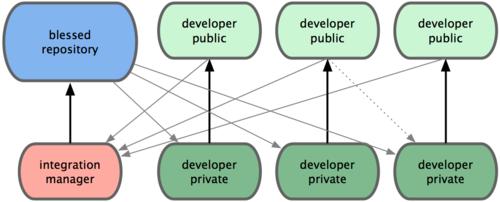
\includegraphics[width=.8\textwidth]{git-model-1.png}
  \caption{Integration-Manager Workflow}\label{fig:git-model-1}
\end{figure}

This is a very common workflow, where it is easy to fork a repository
and push your changes into your fork for everyone to see. One of the
main advantages of this approach is that you can continue to work, and
the maintainer of the main repository can pull in your changes at any
time. Contributors don't have to wait for the DHBB coordinator to
incorporate their changes.

A variant of a multiple-repository workflow is shown in
Figure~\ref{fig:git-model-2}. It is generally used by huge projects
with hundreds of collaborators but can be adopted by DHBB. Various
integration managers are in charge of certain parts of the repository;
they are called lieutenants. All the lieutenants have one integration
manager known as the benevolent dictator. The benevolent dictator's
repository serves as the reference repository from which all the
collaborators need to pull. 

\begin{figure}[thbp]
  \centering
  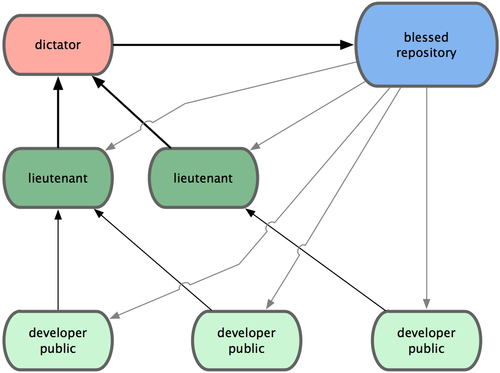
\includegraphics[width=.8\textwidth]{git-model-2.png}
  \caption{Dictator and Lieutenants Workflow}\label{fig:git-model-2}
\end{figure}

This kind of workflow is not common for git users but can be useful in
very big projects or in highly hierarchical environments, as it allows
the project leader (the dictator) to delegate much of the work and
collect large subsets of code at multiple points before integrating
them.

These are some commonly used workflows that are possible with a
distributed system like Git, but the reader can see that many
variations are possible to suit your particular DHBB needs. 

% Figure~\ref{fig:git} shows a possible git workflow. A more
% hierarchical workflow is also possible. The Git distributed version
% control system allows for handling this straightforwardly. The
% authors, responsible for creating the raw versions of historical
% data, would create markdown files. These files would then be revised
% by reviewers that submit their final versions to the coordinator or
% request authors revision. The coordinator is responsible for
% maintain the official DHBB git repository.
It is interesting to notice that all these file exchanges are recorded
and the whole process is controlled without any need of sophisticated
workflow systems, following the methodology developed by open sources
communities for open source softwares maintenance. Git is specially
developed to ensure data consistency and keeping track of chances,
authorship and provenance.

This new process will improve the current workflow of DHBB reviewers
and coordinators, since presently there is no aid system for this
task, basically performed using Microsoft Word text files and emails.

% The new database system composed by Markdown files and periodic RDF
% releases can be easily used for accessing data in an efficient
% way. The figure below illustrates the process. CPDOC and their
% collaborators would be responsible for creating Markdown files that
% would be automatically analyzed by a script for generating the RDF
% file, which would be refined and improved. This refined RDF would be
% made available to the web as linked open data, which would allow the
% information to be accessed and improved by the community. On the other
% hand, the RDF would also be stored in a triple store that allows for
% queries using many different GUI configurations (for instance using
% Solr) to easy the access of data stored. This schema follows a modern,
% open and scalable way of sharing and improving the data stored in
% CPDOC.


\section{Conclusion}

In this article we presented a novelty architecture for CPDOC
archives. Our architecture is based on open linked data principal and
open source methodologies and tools. We believe that despite the fact
that CPDOC users will need to me trained to use tools like text
editors, version control and command line scripts, the architecture
will give much more control over the data maintenance. Moreover, the
architecture ensure that new ideas of metadata informations could be
easily incorporated in the data without dependency of database
refactoring. This means that CPDOC team will be less dependency from
FGV's Information Management and Software Development Staff.

Due the lack of space, we did not present our proposals of research on
the use of lexical resources for reasoning in Portuguese in a way to
improve the structure and quality of the DHBB entries.

\bibliographystyle{plain}
\bibliography{sda}

\end{document}



\section{Logics and Ontologies for Portuguese}

One of my main scientific interests is the logics arising from
knowledge representation of texts.  But to discuss logic and reasoning
with logical knowledge representations, in a way that is scalable and
not brittle, we must deal with language seriously. We need to be able
to build up syntactical and semantical representations, so that we can
build logical representations and reason with them, even when these
representations are very superficial.

We would like to repurpose some of the open source machinery developed
for understanding English, to short cut the development of language
processing and reasoning in Portuguese. In particular it would useful
to be able to bootstrap knowledge acquisition in Portuguese using the
knowledge base SUMO to organize meanings/concepts.

The goal of this self-contained, personal, research project is to do
so in the field of biographical features of historical characters in
recent Brazilian history. We provide some background and context for
the project, before a schematic description.


\section{Background: Textual Inference Logic at FGV}

Our research project started in August 2010. Financial support has
been provided by FGV, which has paid for visits by Dr. de Paiva and
Dr. de Melo to FGV.  The first visit by Dr. de Paiva was in September
2010 and the second by Dr. de Paiva and Dr. de Melo was in November
2011. To make the second visit more productive, we organized a
workshop at FGV titled ``Logics and Ontologies for
Portuguese''.~\footnote{\url{http://emap.fgv.br/events/nlp-2011/}.}
FGV has also paid for trips of Dr. Alexandre Rademaker for his
participation in international conferences.

In more detail, Alexandre Rademaker and I started talking about the
research in reasoning from language when he was doing his internship
with Natarajan Shankar at SRI, Menlo Park in 2009. I was working for
Cuil, Inc and got him interested in the idea of Processing Natural
Language to obtain logical formulas (in Description Logic, the subject
of his doctoral work) and in obtaining a reasoning logical framework
out of free-form text, using the work I had been doing at Xerox PARC's
Natural Language Technology and Theory (NLTT) previously.

Most of the work in processing natural language has been done for
English, but adapting some of this work to Brazilian Portuguese should
not be too difficult, we reasoned in 2010. While the work I did at
PARC encompassed a whole pipeline from reading text to using the
representations built in applications such as Question Answering or
Summarization, since we were promised the use of PARC's codebase for
academic purposes, our initial intention was simply to supply the
necessary Portuguese language resources to complement the PARC system,
as far as the more logical tasks were concerned.
 
To this end I visited the FGV in late 2010 for some brainstorming
sessions on what would be the most useful applications of NLP in
Portuguese, as far as FGV objectives were concerned. I tried to map
local Portuguese resources and tried to uncover relevant possible
collaborators. I also gave three lectures on the subject of what I
wanted to do and how (in very loose terms) this could be achieved.
 
From these conversations and given that fact that I was hoping to get
a Xerox PARC license to use their system XLE-Bridge for our project,
we decided that, as first step, we needed a lexical resource such as
Princeton's WordNet for Portuguese.

We knew there were already in existence three other projects
(\cite{wn1, wn2, wn3}) trying to provide a Portuguese WordNet, so we
first assumed we would be able to join one of these projects and use
their resources. Unfortunately this was not possible. None of the
groups wanted to produce open source code, freely downloadable, which
seemed to us the only way to grow up and keep improving this kind of
resource.  Thus we engaged in a project of our own, named
OpenWordNet-PT~\cite{GWA:2012:VCP:AR}, (or Open WordNet in
Portuguese), as none of the previous proposals seemed to want to post
openly and allow downloading of the resources they develop. Our
project and prototype were funded by FGV itself.

We came across the Global WordNet Association (GWA) and felt inspired
to obtain a small core version of a Portuguese WordNet by manually
translating the core concepts of the original Princeton word net, a
method suggested by the GWA. Through recommendation of Adam Pease,
then at Rearden Commerce, we were introduced to Gerard de Melo's work
on the Universal WordNet \cite{}, a large-scale multilingual lexical
database that seemed very relevant to our project. Universal WordNet
(UWN) organizes over 800,000 words from over 200 languages in a
hierarchically structured semantic network, providing over 1.5 million
links from words to word meanings. Amongst these 200 languages
Portuguese is considered. This universal wordnet is bootstrapped from
the Princeton WordNet using graph-theoretic techniques, the core of de
Melo's doctoral work with G. Weikum at MPI. De Melo's multilingual
universal wordnet has a high level of precision and coverage, and it
can be useful in applied tasks such as cross-lingual text
classification. We realized that it could be very useful indeed in our
project to bootstrap the resources necessary to creating our version
of a Portuguese WordNet and decided to invite Gerard to talk about his
research at FGV in Rio de Janeiro in November 2011.

After a week of intense discussions and many hours of lecture
preparation and presentation in Rio, it was decided that Gerard would
prepare a big file from the original UWN, which I called a
``projection" of the universal worldnet, consisting of the synsets in
Portuguese and Spanish, which we would then manually curate, with the
help of Rafael Hauesler, Alexandre's intern at FGV. We also had
beginnings of discussions of how the data could and should be used,
but no conclusive decisions were taken.

Later on Alexandre Rademaker went to the Global WordNet Association
meeting in Japan and talked about the project, the paper is in the
{\it Proceedings of Global Wordnet Conference} \cite{}.  Recently
Francis Bond added the OpenWordNet-PT to his online interface to many
open wordnets ``Open Multi-lingual Wordnet (1.0)".

Thus our first version of OpenWordNet-PT launched in August 2012 with
7422 adjectives, 55951 nouns, 1726 adverbs and 7155 verbs. It can be
searched online and/or downloaded at the site. It has a collection of
problems, as any first version of a resource, for example we have some
duplicates, as a by-product of how the entries (sunsets) were
created. But all in all it is a remarkable result for such a short
project, so far.

\section{Context for Resources and Reasoning}

In the long term, as results from this project, we envisage a
collection of several modules, helping to produce logical forms from
sentences, including, perhaps, Brazilian Portuguese versions of
WordNet, SUMO, NOMLEX~\cite{nomlex}, VerbNet~\cite{verbnet}, specific
ontologies (of e.g. politicians roles) for the domain as well as a
lexicon of multiword expressions adapted to the domain we want to
concentrate on, historical biographies. In the meanwhile we believe we
need to organize:
%The contents of the modules are:

\begin{enumerate}

\item Online searchable Corpora. The archives of FGV plus collections
  of texts freely available, preferably with various genres.

  In particular the would like to process a downloaded version of the
  Portuguese Wikipedia to make side by side comparisons with the CPDOC
  dictionary of historical characters (DHBB). Both Wikipedia infoboxes
  and its internal links network can be used to induce similar
  collections in the CPDOC dictionary, if there is a great
  intersection of the resources, which we believe there will be. For
  general comparison and baseline we can use other corpora available
  from NILC~\footnote{\url{http://www.nilc.icmc.usp.br/}}, for
  instance.

\item WordNet-like lexical database. There are several proposals for
  WordNet-like ontologies for Portuguese, but as described above, none
  seem to work for us. The papers by Teixeira et al and Oliveira et al
  \cite{Oliveira2008,teixeira2010} describe the situation (as in 2010)
  and provide some links.
  
  As mentioned above we now have a first version of our own resource,
  OpenWN-pt, freely available at \url{} and downloadable, but whose
  quality and accuracy is not, as yet, measured. Producing credible
  measurements of the quality of OpenWN-PT is one of our first goals
  in the new project.

\item VerbNet-like lexical knowledge base. We believe a Brazilian
  attempt at a VerbNet-like resource is under development at NILC,
  USP-SC, but no promises of open access have been made.
 % effort for Portuguese, yet, despite the fact that the main architect
 % of VerbNet~\cite{verbnet}, Karin Schuler, is Brazilian. 
  
  Also we plan to partner with the group of Prof. Leonel Alencar from
  the Universidade Federal do Cear\'a to work on the more syntactical
  aspects of our project and they apparently are planning a different
  version of a Portuguese VerbNet. If this turns out to be the case,
  we hope to be able to use it in our research.
 
\item Named Entity Recognizer. Apparently, there are many entity
  recognizers available for Portuguese. There was a couple of
  competitions between these, HAREM is the name of the competition,
  lead by Diana Santos. The second edition of the competition has
  edited a book, and slides for the presentations can be found at the
  competition
  website.~\footnote{\url{http://www.linguateca.pt/aval_conjunta/HAREM/EncontroSegundoHAREM.html}}
  More about HAREM at \url{http://www.linguateca.pt/HAREM/}.
  
  But other recognizers such as Rembrandt \cite{}(\url{}) and
  Wikipedia Miner seem also interesting possibilities. We need to
  decide which recognizer we will be wanting to use and then test and
  measure its coverage and accuracy.
  % A possible collaborator of our project Dr Christian Aranha has
  % experience with NERs in Portuguese, but since Dr Aranha has a
  % small
  % company selling language tools and we want everything in our
  % project
  % to be freely available we have not yet uncovered how to make the
  % proposed collaboration work.
 
\item 
  % SUMO in Portuguese. We believe that our students and contributors
  % can, mostly, deal with our chosen ontology SUMO and its
  % development environment Sigma in English, but we plan to translate
  % parts of the domain ontology specifically dedicated to historical
  % figures to Portuguese. More importantly
  We hope to leverage SUMO as a formal {\em lingua franca}, to help
  validate our automatic translation of Princeton's English WordNet
  into Portuguese.

  SUMO has the beginnings of a domain ontology dedicated to historical
  figures, started as part of a project to cover all of Wikipedia
  infoboxes concepts in SUMO under Adam Pease's direction. Many of the
  Wikipedia infoboxes are about historical figures. Infoboxes contain
  only some basic information about historical figures, like name,
  date of birth, date of death, official title or position and
  predecessor and successors in that position. We reckon that
  recognizing this kind of information in all biographies in the FGV
  dictionary will help make it more informative, as it will provide
  means of navigation towards both other people in similar positions
  or to the places and times where events happened. Eventually we
  would like to bring in also the events themselves and relationships
  between them, but the first step ought to be simply connecting
  people with their less controversial data, such as data and place of
  birth and death.

  SUMO has already a specialized small ontology called Biography.kif
  created for the purpose of mapping Wikipedia's infobox biographical
  information to SUMO, but many of the positions/professions in
  Wikipedia info boxes are not yet mapped into SUMO concepts.  SUMO
  also has the basic translations of its main concepts (around a
  thousand) to Portuguese, but we believe this is not enough for the
  process of cleaning up and improving our biographical data in
  Portuguese. While we could, in principle, translate the whole SUMO
  ontology to Portugues, it is not clear to us (a this stage) that
  this would be a good use of resources.

  We hope that {\bf triangulation} between the data in the OpenWN-PT,
  the data in the FGV dictionary DHBB, the data in the Portuguese
  Wikipedia and the data in the English Wikipedia will help us improve
  the quality of the the resources.
  
  %if we can have the human support we are hoping for. 
  For the triangulation of the data itself we hope to count on the
  expertise of Dr Gerard de Melo, who visited FGV in Nov 2011 and
  seems enthusiastic about the project. Dr de Melo brings a formidable
  experience with the lexical knowledge base YAGO, where electronic
  dictionaries and thesauri in several languages were used with the
  backbone of WordNet synsets taxonomies as a means for the
  construction of multilingual WordNets and a generic ontology
  extracted from Wikipedia.

\item A small side project that we are also engaged in is a collection
  of small hand-curated lexicons such as NOMLEX-BR. NOMLEX in English
  is a well-established project out of New York City University that
  has become a de facto baseline for the study of nominalizations in
  many languages. The project is open source and freely distributable,
  so we intend to provide our own (preliminary) version of NOMLEX-BR
  as they do, as soon as possible.  Nominalizations are important for
  knowledge representation as ontologies tend to concentrate their
  content in noun hierarchies, paying much less attention to verbs,
  which usually correspond to processes. Nominalizations (sometimes
  called deverbals in the AI literature) are an important mechanism
  that languages have to transform verbs into corresponding
  nouns. Investigating how nominals (or deverbals) work both in
  English and in Portuguese will improve SUMO itself and it will help
  us with the modeling of events in language, in general.
  
\item Finally we want to explore comparing and combining our system
  with complementary frameworks and knowledge sources.
  Prof. Dr. Vladia Pinheiro, another possible collaborator in the
  project, has created an ontological representation based on a
  common-sense knowledge base called ConceptNet. We wondered if we
  could set up a joint project with Dr Pinheiro to have her systems
  SIA (Semantic Inferialist Analyzer) and SIM (Semantic Inferialist
  Model) compare Wikipedia violent events in Brazilian History to her
  corpus of occurrences.  Dr Pinheiro's system at the moment is tuned
  to deal with crime in the streets of Fortaleza, and has vocabulary
  to deal with these kinds of violent events.
\end{enumerate}

Among the resources we do plan to investigate as the project develops,
as we know they will be needed at some later stage are:

\begin{enumerate}
\item Temporal expressions recognizers
\item Geographic and spatial expressions recognizers
\end{enumerate}

This is a fairly ambitious proposal, but it can be cut down to size,
to yield immediate ``low hanging fruit''. In the following section we
describe in more detail where we plan to concentrate the immediate
efforts of this collaboration.

% To analyze FGV's historical texts, we would need an LFG (Lexical
% Functional Grammar) for Portuguese, coupled with some lexical
% resources. In particular we need some collections of texts reasonable
% clean (corpora), we need electronic dictionaries and thesauri
% (Jspell~\footnote{\url{http://www.jspell.com/}} and/or
% aspell~\footnote{\url{http://aspell.net/}} might be enough), we need a
% morphological analyzer and a named entity recognizer. We also need
% lexical resources like a Portuguese versions of WordNet, NOMLex and
% VerbNet.
% These resources are not particularly easy to obtain or to put to work
% together. Some of the resources are independent and could be pursued
% in parallel.

\section{Resources for Reasoning}

Our new joint collaboration ``Resources and Reasoning" has four main
immediate goals, namely:

\begin{enumerate}
\item Measure and improve the accuracy of our own OpenWordNet-PT;

\item Choose and implement a version of named entity recognition and
  of a tokenizer for Brazilian Portuguese;

\item Create an ontology of salient concepts associated with
  historical biographies in SUMO and show its suitability for
  modelling FGV's Dictionary of Brazilian Historical Biographies, the
  DHBB.

\item Demonstrate the feasibility of a prototype for reasoning about
  relationships between historical characters in the DHBB, using
  SUMO-Sigma and the resources we have created.
\end{enumerate}

Our main goal is the last one, where we hope to do some logical
reasoning using the ontology created in item 3.

\section{Brazilian Dictionary of Historical Biographies Mining}

The main application we envisage for our work in OpenWordNet-PT is
simple, but groundbreaking.  We want to read the entries in the DHBB
and extract from them the main SUMO concepts referenced.  Using these
main SUMO concepts we want to bootstrap a fledgeling Ontology of
Historical Biographies, already started and documented in the
Development section of SUMO.  From the analysis of the SUMO concepts
uncovered in the biographical entries, we want to discover new
relationships between the historical characters described in the DHBB.

Here are some examples of the kinds of questions that this association
of text of biography entry with collections of SUMO concepts will
allow us to answer:

\begin{itemize}
\item Amongst Brazilians first rank politicians how many are from Sao
  Paulo?
\item Has the proportion of ``Paulistas'' increased of decreased since
  the 1930's? SInce 1965 when Brasilia became the Capital of Brazil
  has the proportion changed?
\item What are the important Brazilian political families,
  corresponding to the Kennedy's, the Bush's, etc?
\item What are the prevalent occupations among Brazilian historical
  figures? Are they all lawyers by training?
\item Are there Universities or Colleges who clearly create
  ``political leaders''?
\item Are there Universities or Colleges who clearly create ``economic
  leaders'' or entrepreneurs?
\end{itemize}

To get to the stage of asking and answering these questions we need
first to actually provide the so-far potential mapping from words in
Portuguese to SUMO concepts.

There is such a mapping in English, one of the reasons SUMO is a good
choice for us. This mapping is described in ``Linking Lexicons and
Ontologies: Mapping WordNet to the Suggested Upper Merged Ontology'',
Ian Niles and Adam Pease
(http://home.earthlink.net/~adampease/professional/Niles-IKE.pdf). Since
Portuguese synsets are linked to English synsets we can possibly use
this composite mappings, but the disambiguation problem might hit us
hard. We need to check.

If the composite mappings work, via our OpenWordNet-PT and the ability
to relate synsets in Portuguese to synsets in English, we can perhaps
`inherit' a high quality, hand-coded, WordNet to SUMO mapping.

To be able to use this mapping we need first to be able to tokenize
our sentences and we need to be able to detect ``named entities" in
our corpora. We also need to recognize "compound expressions" that are
essential to our domain such as ``deputado federal" or ``primeira
dama". I believe that producing lexicons for this specific domain
should be feasible in a one-year long full time project, which may
take longer, if done in short spells.

Many more lexical resources would be helpful for reasoning about
free-form text. We mention here two other resources that we have
started working on, a Portuguese version of NOMLEX and a Portuguese
version of existential change verbs. Even if we are using superficial
(not deep) processing of the language, that is, even if we do not
parse sentences and try to find all the information conveyed, it is
rather essential to distinguish verbs that signify non-existence of
concepts. An example would be ``The meeting was cancelled''. In the
context of this utterance there is no real meeting, as that was
cancelled, but the usual meddling of the sentence would create a
concept corresponding to this nonexistent meeting. This non-existence
needs to be accounted for even in shallow processing of language.

\section{Summary}

This unusual proposal for a part-time Senior Visiting Professorship is
based in part on a research program me already in course with
Prof. Alexandre Rademaker.

This research programme aims at developing tools and resources for
Brazilian Portuguese that would allow us to construct and reason with
logical forms extracted from unstructured text. The research program
me was originally called ``Textual Inference Logic'' (TIL) and it is
now called ``Resources and Reasoning in Portuguese''.

The goals are the same, the methods have hardly changed, but we are
getting clearer on what we can accomplish given a certain amount of
time. We aim to use SUMO and its theorem prover Sigma as ontology
building and improving tools for our knowledge bases based on CPDOC's
Historical Dictionary of Brazilian Biographies (DHBB). The project has
already produced a preliminary version of a Brazilian Portuguese
lexical base OpenWN-PT in the style of Princeton's WordNet and we plan
to improve this lexical base and use it to reason about the
biographies of historical politicians in the DHBB.


% Also some corpora available from
%   Linguateca~\footnote{\url{http://www.linguateca.pt/}}. In
%   particular, Brazilian colleagues have worked hard to produce TEP, an
%   electronic thesaurus for Brazilian Portuguese, \cite{mazieroetal}.

% \item Wordnet lexical-semantic database. There are several proposals for
%   WordNet-like ontologies for Portuguese. The papers by Teixeira et al
%   and Oliveira et al \cite{Oliveira2008,teixeira2010} describe the
%   situation and provide links.

% \item VerbNet-like lexical ontology. We have not seen a similar effort
%   for Portuguese, yet. But the main architect of VerbNet (Karin
%   Schuler) is Brazilian, she might be interested in helping out.

% \item Morphological analyzer. There are apparently many available.  So
%   much so that there is/was a couple of competitions to discover the
%   best one, organized by Diana Santos. A preliminary write-up is
%   available from \cite{santos2003}. Perhaps PALAVRAS is a good
%   option?~\footnote{\url{http://beta.visl.sdu.dk/visl/pt/parsing/automatic/}}
 
% \item Named Entity Recognizer. There are apparently many available. So
%   much so that there is/was a couple of competitions to discover the
%   best one, HAREM is the name of the competition, lead by Diana
%   Santos. The second edition of the competition has edited a book, and
%   slides for the presentations can be found at
%   \url{http://www.linguateca.pt/aval_conjunta/HAREM/EncontroSegundoHAREM.html}.
%   More about HAREM at \url{http://www.linguateca.pt/HAREM/}.

% \item A LFG grammar. If we have an LFG grammmar we might be able to
%   use the XLE(Xerox Language Engine) directly, hence we do not need a
%   (deep) parser of our own. Similarly we might be able to use the
%   transfer semantics and the AKR (abstract knowledge representation)
%   creation facilities.

% \item Anaphora Resolution. This is required for dealing with more than
%   one sentence, as we need to recognize the entities referred to in
%   previous sentences.
% \end{enumerate}

% Note that if we do not have an LFG grammar, then we need a parser, a
% semantics module and some sort of knowledge representation module,
% which brings the numbers from six to nine modules.  The corresponding
% system for English, together with some lessons learned, has been
% described in \cite{depaiva:LFSA}.

% Among the resources we do not investigate, despite knowing that they
% will be needed at some later stage are:

% \begin{enumerate}
% \item Multiword recognizer 
% \item Temporal expressions recognizer
% \end{enumerate}

% A FrameNet-like resource for Portuguese may also be considered. We hope
% to start with a version of WordNet and some version of VerbNet, that
% we need to construct.






\section{Outline} 
\begin{itemize}
\item Intro
\item Dictionary
\item Using OpenWN-PT, SUMO
\item Categories for Co-Intuitionistic Logic
\end{itemize}

\section{ideas from emails past}

write to Bento, PAlmira Marrafa, Antonio Branco e Vladia and Leonel about helping to improve OpenWN-PT.
Need a email dedicated to reporting issues
Need an email for MArina, Sandra and Henrique.

need to write to Francis asking for 
1. glosses
2. adding an email for reporting mistakes.
Done, reply is good
-----------------
Quality of OpenWordNet-PT
The best strategy is therefore to summarize the description of resources in the end of
such projects and check validity of information in all documents that will be part of
the documentation.
The terminology used in the resource description should be also explicitly defined.
Even the meaning of terms that seem to be basic in the context should be tackled.
For example, synonymic set { synset { is the fundamental building block of wordnets.

The description of the data format in which the resource is provided plays also a
crucial role. As XML has become de facto standard for data interchange, it is natural
to make data available in XML and release the relevant DTD description. Data types
of XML entities and other constraints on the tag content should be also specified.
one of the most successful procedures to control the quality of
linguistic output is to implement a set of validation checks and regularly publish their
results. It holds especially for projects with many participants that are not under the
same supervision. Validation check reports together with the quantitative assessment
can serve as development synchronization points too.

All partners agreed to prepare and update resource description sheet"
for the wordnet they develop. Such a specification should contain at
least: ? description of the content of synset records and constraints
on data types; ? types of relations included together with examples; ?
degree of checking relations borrowed from PWN (see the note about the
expand model below); ? numbering scheme of different senses (random,
according to their frequency in a balanced corpus, from a particular
dictionary, etc.)  ? source of definitions and usage examples; ? order
of literals in synsets (corpus frequency, familiarity, register or
style char- acteristics).

1. All synsets contained in EuroWordNet base concepts have been included to
maximize the overlap between the two projects.
2. The set has been extended based on the proposals of all partners who added
synsets corresponding to the most frequent words in corpora and in various
dictionary definitions for their particular languages.
3. As an additional criterion, several noun synsets that had many semantic rela-
tions in the Princeton WordNet database have been added.

A special mechanism has been adopted to signalize lexical gaps  concepts that
are not lexicalized in a language. Such entries are labeled <NL/> in the BalkaNet
database and they should be ignored when working with a particular wordnet as a
monolingual resource.

Semi-automatic checks that need additional language resources to be integrated
are usually performed by each partner depending on the availability of the resources:
? spell-checking of literals, definitions, usage examples and notes;
? coverage of the most frequent words from monolingual corpora;
? coverage of translations (bilingual dictionaries, parallel corpora);
? incompatibility with relations extracted from corpora, dictionaries, or encyclo-
pedias.
----------------------

 Na linha de tentar construir uma WordNet-BR a partir da EN usando o Google Translation, ja tenho a WordNet 3.0 em RDF em uma triplestore. Esta semana acho que consigo terminar um script para usar o Google translation nos glosses.
 Google APi for glosses still good!
 scraping other wordnets in portuguese?
 email Bento now with stuff available on web and proposal of merge
 
 mas outra possibilidade 'e fazer uma ontologia SUMO de figuras historicas. acho que fazer a ontologia nao 'e dificil, a questao 'e como usar o resultado...
 
 mais uma, usar  verbnet to extract complement verbs and getthe brazilian ones that are the same.
 
 a gente tem a divisao do OpenWB-PT em nouns. verbs, adjectives and adverbs?
 qual e'?
 a gente tem os glosses separados? qdo a gente tem gloss ele aparece no nultilingual?
 
 sentiment lexicon in PT, sentilex
 http://label.ist.utl.pt/pt/downloads-pt.php
 

\section{History.kif, Biography.kif Brazilian Geography.kif?}

Need lists of names, christian and surnames, need list of places and institutions in Brazil. what does wikipedia know?

 I was told by Colin Baker of the framenet beginnings in Juiz de Fora
and indeed it seems a good idea to invite them.

From Information to Understanding: Moving Beyond Search In The Age Of Siri http://tcrn.ch/P3xtAJ
http://techcrunch.com/2012/07/28/from-information-to-understanding-moving-beyond-search-in-the-age-of-siri/
According to Google, the average user visits 22 sites prior to booking travel. Planning a trip can be unnecessarily frustrating and time consuming. What if planning your travel was as easy as interacting with a friend from the area you plan to visit, one whose on-the-ground recommendations cut through the clutter with aplomb, and who knows what you enjoy?

wikipedia on NER: Despite the high F1 numbers reported on the MUC-7 dataset, the problem of Named Entity Recognition is far from being solved. The main efforts are directed to reducing the annotation labor [7] ,[8] robust performance across domains[9][10] and scaling up to fine-grained entity types.[11][12]
At least two hierarchies of named entity types have been proposed in the literature. BBN categories, proposed in 2002, is used for Question Answering and consists of 29 types and 64 subtypes.[5] Sekine's extended hierarchy, proposed in 2002, is made of 200 subtypes.[6]
For traditional NER, the most popular publicly available systems are: OpenNLP NameFinder, Illinois NER system, Stanford NER system, and Lingpipe NER system. The Illinois NER reports 90.6 F1 on the CoNLL03 NER shared task data and the Stanford NER reports 86.86 F1.[16][17]

There are also several publicly available Wikification systems for identifying important expressions in the text and cross-linking them to Wikipedia. Most notably, Illinois Wikification system WM Wikifier and TAGME.

http://xldb.di.fc.ul.pt/Rembrandt/? for Portuguese open source



Cohan Sujay Carlos: The NIST information extraction tasks, especially
MUC and ACE, might be related to what you're working on. You can take
a look at the measures used in those tasks. Here's a paper on some ACE
evaluation metrics:
http://www.itl.nist.gov/iad/mig/publications/storage-paper/ACEXDOC-FinalPaperV3_NIST.pdf -
4 months ago Like


Vineet Yadav Apart from ACE evaluation matrices, you can also look at
MUC evaluation matrices(http://acl.ldc.upenn.edu/M/M92/M92-1002.pdf,
http://acl.ldc.upenn.edu/M/M93/M93-1007.pdf). You can look at Diana
Maynard(http://www.dcs.shef.ac.uk/~diana/) paper on evaluation of
information extraction system(Metrics for Evaluation of Ontology-based
Information Extraction). Diana Maynard works in University of
Sheffield on GATE information extraction
system(http://gate.ac.uk/). You can look at GATE evaluation matrics
(http://gate.ac.uk/sale/tao/splitch10.html#x14-25900010.1) and GATE
balanced metric score pluggin(
http://gate.ac.uk/sale/tao/splitch10.html#x14-28300010.6). You can
find more information about GATE balanced metrics score plugin in
Diana paper "Metrics for evaluation of ontology-based information
extraction" and "Benchmarking ontology-based annotation tools for the
semantic web." ). If you are creating training dataset for information
extraction system,then apart from precision, recall calculation, you
can also calculate inter-annotator agreement between the
annotators. you can use Cohen Kappa
agreement(http://en.wikipedia.org/wiki/Cohen\%27s_kappa) or
krippendrop alpha
(http://en.wikipedia.org/wiki/Krippendorff\%27s_Alpha) to calculate
inter-annotator agreement between different annotators.




The research proposed here is an extension of the linear functional programming 
paradigm. Most of the work concerning linear functional programming has used as 
its basic language the system of Intuitionistic Linear Logic, the fragment 
considered by Lafont. For this fragment, since derivations have a single 
conclusion, it is easier to consider a Natural Deduction formulation, and hence 
the analogy with standard functional programming is clearer. we intend to develop 
the computational interpretation of FILL. The challenge comes from the fact that 
since derivations in the system have multiple conclusions (to be thought of as 
terms to be evaluated in parallel) the concept of Natural Deduction becomes much 
more involved. There are a few attempts in the literature at notions of multiple 
conclusions Natural Deduction, but none of the solutions proposed to date seems 
satisfactory. The motivation for seeking a multiple conclusion system seems 
clear: this corresponds to an intrinsically parallel version of (linear) 
functional programming and as such it will help with resource control in a 
parallel-based environment. In other words FILL has potentially the ability 
to initiate a new style of functional programming where parallelism is directly 
built into the derivations. We should try to develop this idea into a working 
implementable system either along the lines of Mackie's linear programming 
language Lilac, \cite{Mackie91}, or along the lines of an extended version of 
D. Miller's logic programming language Forum, \cite{Miller94}, which is based 
on linear logic.

Some work has already been done on FILL. The original presentation of the system, 
in \cite{HylanddePaiva93}, had a mistake and the system as presented did not enjoy 
the cut-elimination property. In a paper by Bra\"{u}ner and de Paiva, 
\cite{BraunerdePaiva96}, as well as correcting the mistake in the original paper 
and extending the system to deal with exponentials, we introduced a different 
formal system describing the intuitionistic character of FILL and provided a full 
proof of the cut elimination theorem. The idea of a notion of dependency between 
formulae within a given proof is the basis of our new formal system and it seems 
of independent interest. For example, the formalisation of this notion seems a 
challenge to formalisms like Milner's new action calculi. The procedure for cut 
elimination applies to Classical Linear Logic, and we can (with care) restrict our 
attention to the subsystem FILL. Historically, our work on FILL grew out of a 
search for a fragment of Classical Linear Logic with a polynomial time cut 
elimination algorithm, analogous to the aim of Girard's Light Linear Logic, 
\cite{Girard94}. 

Having solved the problem of how to formulate the pure logic for FILL in a way 
that guarantees cut elimination, we are keen to tackle the other problem raised 
in the original paper. To quote the last paragraph of \cite{HylanddePaiva93}:
\begin{quote}
{\em It still remains to give a satisfactory account of the computational meaning 
of the term calculus for FILL. With other colleagues we have been trying to give 
an interpretation in terms of processes, but we rather hope that a number of 
different interpretations will emerge. We should like to end by recording our 
belief in the significance of FILL. It seems to provide a context for considering 
different interpretations of functional programming, and as such to deserve 
further attention.}
\end{quote}
The goal of the project will be to give a computational account of FILL. This 
includes considering the following problems: 
\begin{itemize}
\item 
A Curry-Howard interpretation of the pure logic as given by Bra\"{u}ner and 
V. de Paiva, \cite{BraunerdePaiva96}, should be developed. This includes 
obtaining an appropriate notion of reduction. The questions of operational 
semantics, evaluation strategies can then be addressed. Abramsky's proof-terms 
will not do as they do not deal with linear implication explicitly, but instead 
has negation built-in in a way such that it automatically is involutive.
\item 
Strong normalisation and Church-Rosser results for the Curry-Howard 
interpretation of FILL should be proved.
\item 
A non-trivial sound denotational semantics should be given in a way that explains 
the characteristic features of FILL.
\item 
The constructive nature of FILL should be clarified considering the questions of 
Church-Rosser and denotational semantics. This should be compared to the 
intuitionistic nature of Intuitionistic Linear Logic and contrasted to the 
non-intuitionistic, but constructive, nature of Classical Linear Logic. 
\item
The issue of recursion in the linear version of PCF dealt with in Bra\"{u}ner's 
Ph.D. dissertation should be considered in the more complicated setting of a term 
calculus for FILL.
\item 
A comparison with the classical system of M. Parigot, \cite{Parigot92}, should 
be attempted. In particular using the ideas of the $\lambda\mu$ calculus we ought 
to obtain classical linear logic from FILL. 
\item 
Several recent attempts at generalised notions for concurrency e.g. $\pi$-calculus 
and actions structures seem to use linear logic notions. It would be interesting 
to investigate whether FILL's notion of dependency between formulae (types) can be 
captured by action calculi and whether FILL can shed some light on the categorical 
modelling of such calculi. There is some work in progress in Edinburgh along these 
lines.
\end{itemize}


